\documentclass[french]{article}

\usepackage{mathtools, bm}
\usepackage{amssymb, bm}
\usepackage[utf8]{inputenc}
\usepackage[T1]{fontenc}
\usepackage{babel}
\usepackage{amsmath}
\usepackage{graphicx}
\usepackage{eso-pic}
\usepackage{fullpage}
\usepackage{ulem}
\usepackage{ntheorem}
\usepackage{xcolor}
\usepackage{titlesec}
\usepackage{stmaryrd}
\usepackage{calrsfs}
\usepackage{textcomp}
\usepackage[left=2cm,right=2cm,top=2cm,bottom=2cm]{geometry}
\theorembodyfont{\upshape}
\theoremstyle{break}

\definecolor{rougetitre}{RGB}{240, 23, 23}
\definecolor{dorure}{RGB}{147, 127, 8}
\definecolor{dorure2}{RGB}{135, 100, 6}
\definecolor{dorure3}{RGB}{102, 68, 0}
\definecolor{bleuturquoise}{RGB}{30, 81, 122}
\definecolor{vertturquoise}{RGB}{15, 127, 110}
\definecolor{fond}{RGB}{240,240,240}

\titleformat{\section}
   {}% apparence commune au titre et au numéro
   {}% apparence du numéro
   {1em}% espacement numéro/texte
   {\LARGE}% apparence du titre

\titleformat{\subsection}
   {}% apparence commune au titre et au numéro
   {}% apparence du numéro
   {1em}% espacement numéro/texte
   {\large}% apparence du titre

\titleformat{\subsubsection}
   {}% apparence commune au titre et au numéro
   {}% apparence du numéro
   {1em}% espacement numéro/texte
   {\underline}% apparence du titre

\title{Projet base de données}
\author{Julie SAOULI, Maxime GOURGOULHON, Pierre BOUVIER, Geoffrey TANGUY, Jérôme THÉATE}
\date{ENSIMAG | Enseignant encadrant : M. Christophe BOBINEAU | 2017 - 2018 }
\makeatletter 
\begin{document}
\renewcommand*\contentsname{\huge{Table des matières\vspace{1cm}}}
\begin{titlepage}
\begin{center}
\text{  }\\
\text{  }\\
\text{  }\\
\text{  }\\
\textcolor{dorure3}{\textbf{{\fontsize{45}{45}\selectfont Projet Base de Données}}}\\
\vspace{0.5cm}
\textcolor{dorure3}{\textbf{\LARGE{COMPTE-RENDU}}}
\end{center}
\vspace{3cm}
\begin{center}
\makebox[\textwidth]{\includegraphics[scale = 1, width=\paperwidth,height=10cm]{proverbe2.jpg}}
\end{center}

\vspace{4.0cm}
\begin{center}
Julie SAOULI \hspace{1.5cm} Maxime GOURGOULHON  \hspace{1.5cm} Pierre BOUVIER
\end{center}
\\
\hspace{4.2cm} Geoffrey TANGUY \hspace{3cm} Jérôme THÉATE
\\
\vspace{0.2cm}
\begin{center}
\large{\@date}
\end{center}
\end{titlepage}
\clearpage

\begin{Large}
\tableofcontents{}
\end{Large}
\clearpage







\textsc{\textcolor{dorure2}{\LARGE{Introduction}}}
\addcontentsline{toc}{section}{Introduction}
\vspace{1cm}

L'agence de voyage \textsc{awhy}, forte de son succès, entreprend sa transformation numérique.

Elle tient à numériser ses outils de gestion : CRM, suivi de voyage, etc., et base de données. Tout en concervant une étroite collaboration avec ses entreprises partenaires. De ce fait, certaines règles d'implémentation devront être respectées afin d'assurer le fonctionnement des outils numériques entre tous les partenaires.\\

Dans le cadre du développement de la société \textsc{awhy}, nous avons été mendaté afin de réaliser la conception et l'implémentation de leur base de données. Ce rapport vous apportera les outils necessaires à la compréhension de la conception de cette base de données. Et vous permettra en outre de prendre connaissance des enjeux et des difficultés qui ont permis de privilégier certains axes de réflexion.
Enfin, vous y trouverez certains détails quant à nos choix d'implémentation, nous permettant de mettre en valeur et d'exploiter le potentiel de la base de données.










\noindent\textsc{\textcolor{dorure2}{\section{Conception de la base de données}}}

\textsc{\textcolor{dorure}{\subsection{Propriétés élémentaires}}}
\vspace{0.3cm}

\{ nomVille, pays, nomLieu, adresseLieu, descriptifLieu, prix,
idCircuit, descriptif, villeDépart, paysDepart, villeArrivee, paysArrivee, nbJoursTotal, prixCircuit, dateDepartCircuit, nbPersonnes, ordre, nbJours, nomHotel, adresseHotel, nbChambresTotal, prixChambre, prixPetitDejeuner, numDossier, idClient, typeClient, anneeEnregistrement, nomClient, prenomClient, adresseClient, emailClient, telClient, datePaiement, infoPaiement, nbChambres, dateDepartHotel, dateArriveeHotel, dateVisite, nbPersonnesVisite, nbChambresReservees, nbPetitDejReserves, numDossierReservation \}




\vspace{0.3cm}
\textsc{\textcolor{dorure}{\subsection{Dépendances fonctionnelles}}}
\vspace{0.3cm}





\textsc{Issues du sujet :}
\vspace{0.3cm}

\begin{small}
\noindent nomLieu, nomVille, pays → adresseLieu, descriptifLieu, prix\\
\noindent idCircuit → descriptif, villeDepart, paysDepart, villeArrivee, paysArrivee, nbJoursTotal, prixCircuit\\
idCircuit, dateDepartCircuit → nbPersonnes\\
idCircuit, ordre → nomLieu, nomVille, pays, nbJours\\
nomHotel, nomville, pays → adresseHotel, nbChambresTotal, prixChambre, prixPetitDejeuner\\
\end{small}

\textsc{Issues de notre sgbd:}
\vspace{0.3cm}

\begin{small}
\noindent idClient → nomClient, prenomClient, typeClient, adresseClient, emailClient, telClient, annéeEnregistrement\\
numDossier, idCircuit, dateDepartCircuit → nbPersonnesCircuit\\
villeDepart, paysDepart → nomVille, pays\\
villeArrivee, paysArrivee → nomVille, pays\\
numDossier, nomHotel, nomVille, pays, dateDepartHotel, dateArriveeHotel → nbChambresReservees, nbPetitDejReserves\\
numDossier, nomLieu, nomVille, pays, dateVisite → nbPersonnesVisite\\
numDossierReservation → datePaiement, infoPaiement\\
numDossierReservation → idClient
\end{small}




\vspace{0.3cm}
\textsc{\textcolor{dorure}{\subsection{Contraintes de multiplicité}}}
\vspace{0.3cm}




\noindent numDossier $-|\twoheadrightarrow$ nomHotel, nomVille, pays\\
nomHotel, nomVille, pays $-|\twoheadrightarrow$ numDossier\\
numDossier $-|\twoheadrightarrow$ nomLieu, nomVille, pays\\
nomLieu, nomVille, pays $-|\twoheadrightarrow$ numDossier\\
numDossier, dateDepartHotel, dateArriveeHotel $\twoheadrightarrow$ nomHotel, nomVille, pays\\
nomHotel, nomVille, pays, dateDepartHotel, dateArriveeHotel $\twoheadrightarrow$ numDossier\\
numDossier, dateVisite $\twoheadrightarrow$ nomLieu, nomVille, pays\\
nomLieu, nomVille, pays, dateVisite $\twoheadrightarrow$ numDossier\\
numDossier $-|\twoheadrightarrow$ idCircuit, dateDepartCircuit\\
idCircuit, dateDepartCircuit $-|\twoheadrightarrow$ numDossier\\
idClient $\twoheadrightarrow$ numDossierReservation\\
idCircuit $\twoheadrightarrow$ idCircuit, dateDepartCircuit\\
nomVille, pays $-|\twoheadrightarrow$ nomLieu, nomVille, pays\\
nomVille, pays $-|\twoheadrightarrow$ nomHotel, nomVille, pays\\
nomLieu, nomVille, pays $-|\twoheadrightarrow$ idCircuit, ordre\\
nomVille, pays $-|\twoheadrightarrow$ villeDepart, paysDepart\\
nomVille, pays $-|\twoheadrightarrow$ villeArrivee, paysArrivee




\vspace{0.3cm}
\textsc{\textcolor{dorure}{\subsection{Contraintes autres}}}
\vspace{0.3cm}




\noindent “Un dossier contient au moins une réservation (hôtel, circuit, lieux).”\\
“Il ne peut y avoir deux villes de même nom dans le même pays.”\\
“Un circuit commence par une étape de départ et se termine par une étape d’arrivée. Tout circuit contient au moins deux étapes : le départ et l’arrivée.”\\
“Un client doit avoir au moins une réservation (simulation payée).”\\
“Au paiement, et pour permettre la réservation du voyage, il faut vérifier la disponibilité des hôtels et circuits réservés (nombre de places libres compatible avec nombre de places réservées) ainsi que toutes les contraintes.”




\vspace{0.3cm}
\textsc{\textcolor{dorure}{\subsection{Schéma Entité/Association - \textit{Cf. Annexe 1 pour un agrandissement}}}}
\vspace{0.3cm}





\begin{center}
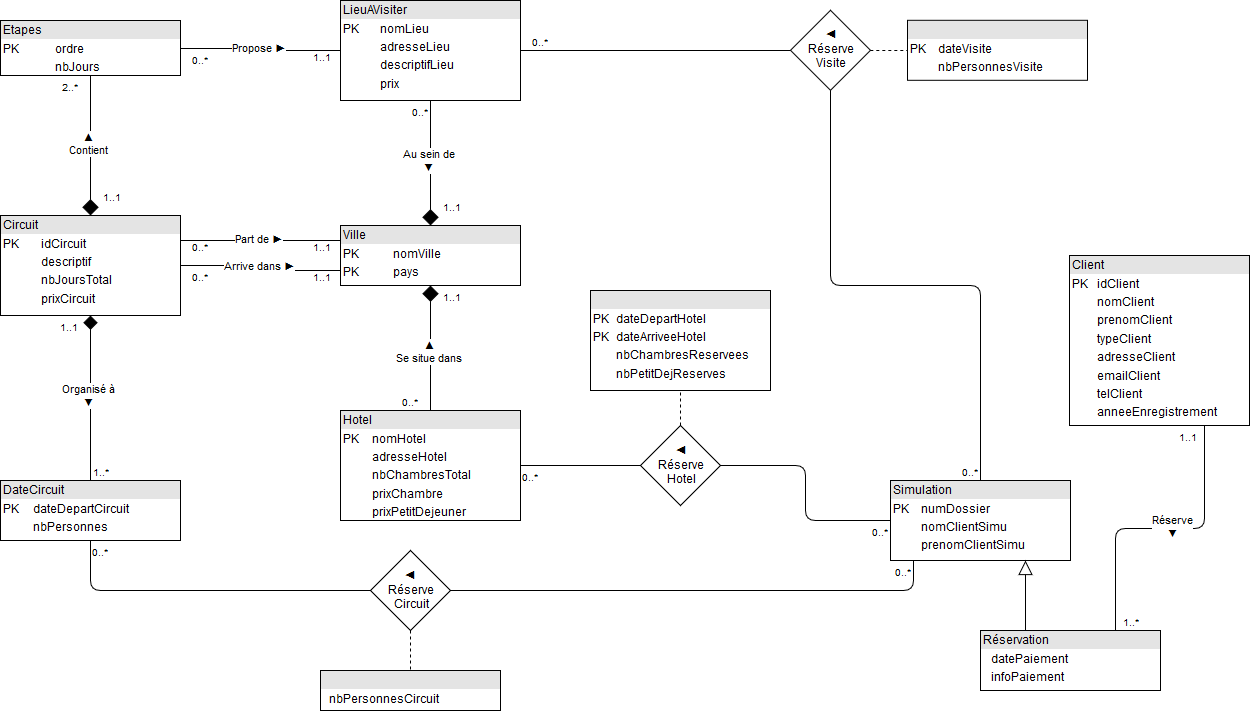
\includegraphics[scale=0.4]{schema_uml.jpg}
\end{center}



\vspace{0.3cm}
\textsc{\textcolor{dorure}{\section{Retrospection sur le projet}}}}
\vspace{0.3cm}


\vspace{0.3cm}
\textsc{\textcolor{dorure}{\subsection{Prise en main du sujet}}}}
\vspace{0.3cm}

Lors de la première séance, nous avons jugé judicieux de travailler ensemble sur la lecture et la compréhension du sujet, mettant en scène une agence de voyage désireuse d'acquérir un \textit{systeme de gestion de base de donnée (SGBD)} performant.

Nous nous sommes dans un premier temps concentré sur l'extraction de toutes les contraintes imposées ainsi que toutes les attentes implicites du client.
Nous avons ainsi pu établir une première liste de propriétés élémentaires \small{(Cf. 1.1)}, de dépendances fonctionnelles \small{(Cf. 1.2)} et de contraintes \small{(Cf. 1.3-1.4)}.
L'édition du schéma entité/association, à partir de l'analyse ainsi faite du sujet a cependant rélévé des incohérences :\\

TODO\\

Suite à cette prise de conscience et à un regain de motivation, nous avons préféré réitérer intégralement le processus de construction de notre SGBD. Operation chronophage mais nécéssaire pour développer notre SGBD sur des fondations solides. Nous avons reprit l'analyse du sujet, l'extraction des dépendances fonctionnelles et des contraintes. Ainsi que l'édition du schéma Entité/Association. Nous nous sommes attardé volontairement sur la vérification de nos résultats et la déduction des formes normales de nos Relations, avant commencer l'implémentation de notre SGBD.\\

Néanmoins, nous avons assez vite réalisé qu'une contrainte imposée par le sujet n'avait pas été perçue à l'issue de nos multiples relectures du sujet : un utilisateur non client peut effectuer des simulations de voyage auprès de l'agence.

Nous avons finalement repris l'analyse de cette partie du sujet, des dépendances fonctionnelles et contraintes associées. Afin d'en déduire notre schéma Entité/Association dans sa version finale.




\vspace{0.3cm}
\textsc{\textcolor{dorure}{\subsection{La gestion du temps}}}}
\vspace{0.3cm}



Les premières séances ont été consacrées à l'analyse du sujet : énumération des propriétés élémentaires, des dépendances fonctionnelles et des contraintes.

Nous avons pris du retard sur l'élaboration du schéma Entité/Association, nous contraignant à repousser d'une semaine la séance de suivie, durant laquelle est effectuée la revue par nos professeurs de notre analyse.

A l'issue de la séance 5 et du suivi, nous avons commencer à consacrer des séances en temps libre pour le projet.
La première nous a permis de reprendre l'analyse du sujet dans son intégralité.

Les séances 6 et 7 ont été consacrées à la mise en place de l'application JAVA, des tables SQL, des requêtes SQL nécessaires à l'application, et au peuplement de la base de données.
Nous avons par la suite consacrer plusieurs heures en tant libre à la finalisation du projet.\\

GANT


\vspace{0.3cm}
\textsc{\textcolor{dorure}{\subsection{La répartition des tâches}}}}
\vspace{0.3cm}



Notre décision de réaliser ensemble la phase d'analyse du sujet, nous a permis de confronter chaque décision à l'avis de tous les membres de l'équipe.

Lors de cette phase cruciale pour notre projet, les interrogations de chacun ont su trouver des réponses. Les différents points de vues et les compréhensions divergentes du sujet, qui nous a semblé sibyllin par quelque fois, ont pu être écoutés puis discutés.

Lors de cette phase nous avons pu exploiter les compétences de chaque membre de l'équipe. Mais également maximiser nos chances de percevoir les erreurs éventuelles, pour mener à bien l'analyse du sujet dont dépendait directement notre projet.


La répartition des tâches s'est concrétisée lors du commencement de l'implémentation physique de notre SGBD.
Nous avons dès lors dissocié la recherche des requêtes SQL, nécessaire au fonctionnement de notre systeme de gestion de base de données, de l'implémentation JAVA visant à créer l'interface graphique faisant le lien entre l'utilisation de notre SGBD et la base de données.\\


TABLEAU DE REPARTITION DES TACHES

\textsc{\textcolor{dorure}{\section{Retours Personnels}}}}
\vspace{0.5cm}

\begin{center}

\begin{minipage}{0.3\linewidth}
\includegraphics[scale = 0.5]{maxime.png}
\end{minipage}
\begin{minipage}{0.5\linewidth}
\center{
--> Impressions <--}\\
\end{minipage}

\vspace{0.5cm}

\begin{minipage}{0.5\linewidth}
\center{
--> Impressions <--}\\
\end{minipage}
\begin{minipage}{0.3\linewidth}
\includegraphics[scale = 0.5]{pierre.png}
\end{minipage}

\vspace{0.5cm}

\begin{minipage}{0.3\linewidth}
\includegraphics[scale = 0.5]{Julie.png}
\end{minipage}
\begin{minipage}{0.5\linewidth}
\center{
--> Impressions <--}\\
\end{minipage}

\vspace{0.5cm}

\begin{minipage}{0.5\linewidth}
\center{
--> Impressions <--}\\
\end{minipage}
\begin{minipage}{0.3\linewidth}
\includegraphics[scale = 0.5]{Geoffrey.png}
\end{minipage}

\vspace{0.5cm}

\begin{minipage}{0.3\linewidth}
\includegraphics[scale = 0.5]{Jerome.png}
\end{minipage}
\begin{minipage}{0.5\linewidth}
\center{
\textsc{Jérôme Théate}\\

Un projet interressant et enrichissant.\\
Un travail en équipe à la hauteur des attentes,\\
qui a permis l'aboutissement du projet grâce à\\
l'implication personnelle de chacun ses membres.}
\end{minipage}

\end{center}

\textsc{\textcolor{dorure}{\section*{Annexe 1 - \textit{Agrandissement schéma Entité/Association}}}}
\addcontentsline{toc}{section}{Annexe 1 - \textit{Agrandissement schéma Entité/Association}}

\begin{center}
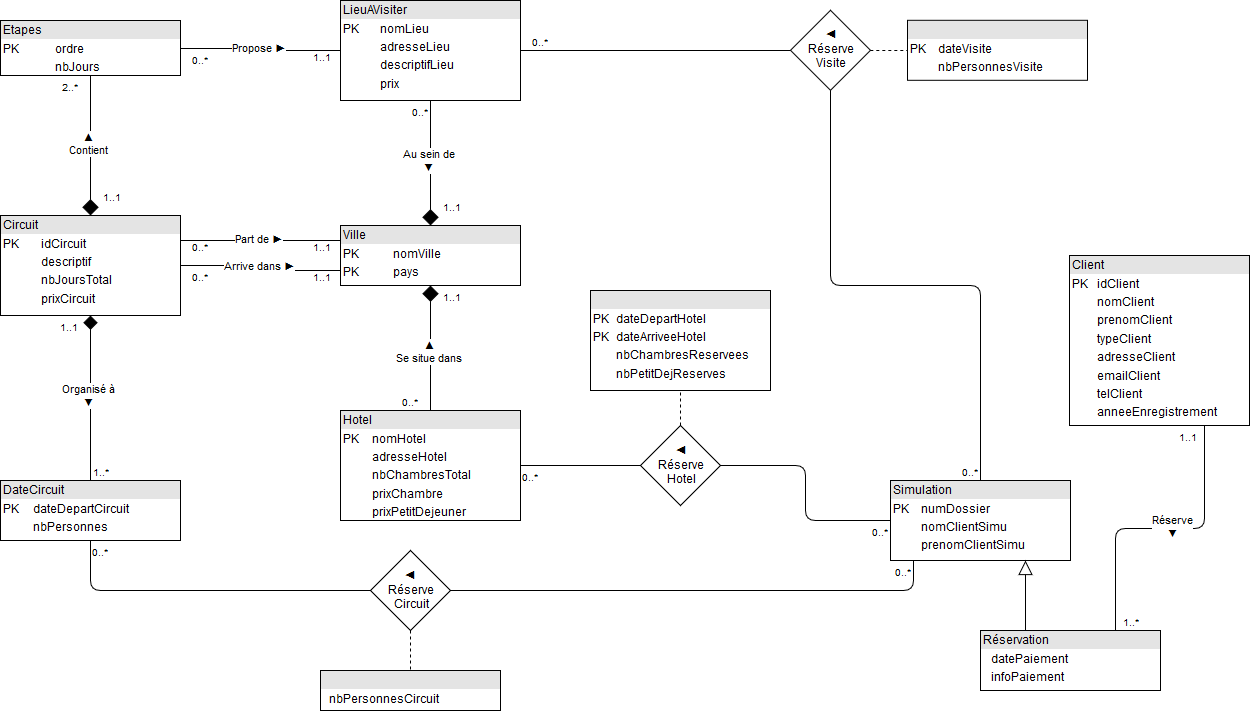
\includegraphics[angle=90, origin=c, width=0.70\textwidth]{schema_uml.jpg}
\end{center}

\end{document}
